%% ut-thesis.tex -- document template for graduate theses at UofT
%%
%% Copyright (c) 1998-2013 Francois Pitt <fpitt@cs.utoronto.ca>
%% last updated at 16:20 (EDT) on Wed 25 Sep 2013
%%
%% This work may be distributed and/or modified under the conditions of
%% the LaTeX Project Public License, either version 1.3c of this license
%% or (at your option) any later version.
%% The latest version of this license is in
%%     http://www.latex-project.org/lppl.txt
%% and version 1.3c or later is part of all distributions of LaTeX
%% version 2005/12/01 or later.
%%
%% This work has the LPPL maintenance status "maintained".
%%
%% The Current Maintainer of this work is
%% Francois Pitt <fpitt@cs.utoronto.ca>.
%%
%% This work consists of the files listed in the accompanying README.

%% SUMMARY OF FEATURES:
%%
%% All environments, commands, and options provided by the `ut-thesis'
%% class will be described below, at the point where they should appear
%% in the document.  See the file `ut-thesis.cls' for more details.
%%
%% To explicitly set the pagestyle of any blank page inserted with
%% \cleardoublepage, use one of \clearemptydoublepage,
%% \clearplaindoublepage, \clearthesisdoublepage, or
%% \clearstandarddoublepage (to use the style currently in effect).
%%
%% For single-spaced quotes or quotations, use the `longquote' and
%% `longquotation' environments.


%%%%%%%%%%%%         PREAMBLE         %%%%%%%%%%%%

%%  - Default settings format a final copy (single-sided, normal
%%    margins, one-and-a-half-spaced with single-spaced notes).
%%  - For a rough copy (double-sided, normal margins, double-spaced,
%%    with the word "DRAFT" printed at each corner of every page), use
%%    the `draft' option.
%%  - The default global line spacing can be changed with one of the
%%    options `singlespaced', `onehalfspaced', or `doublespaced'.
%%  - Footnotes and marginal notes are all single-spaced by default, but
%%    can be made to have the same spacing as the rest of the document
%%    by using the option `standardspacednotes'.
%%  - The size of the margins can be changed with one of the options:
%%     . `narrowmargins' (1 1/4" left, 3/4" others),
%%     . `normalmargins' (1 1/4" left, 1" others),
%%     . `widemargins' (1 1/4" all),
%%     . `extrawidemargins' (1 1/2" all).
%%  - The pagestyle of "cleared" pages (empty pages inserted in
%%    two-sided documents to put the next page on the right-hand side)
%%    can be set with one of the options `cleardoublepagestyleempty',
%%    `cleardoublepagestyleplain', or `cleardoublepagestylestandard'.
%%  - Any other standard option for the `report' document class can be
%%    used to override the default or draft settings (such as `10pt',
%%    `11pt', `12pt'), and standard LaTeX packages can be used to
%%    further customize the layout and/or formatting of the document.

%% *** Add any desired options. ***
\documentclass[onehalfspaced, 12pt, normalmargins]{ut-thesis}

%% *** Add \usepackage declarations here. ***
%% The standard packages `geometry' and `setspace' are already loaded by
%% `ut-thesis' -- see their documentation for details of the features
%% they provide.  In particular, you may use the \geometry command here
%% to adjust the margins if none of the ut-thesis options are suitable
%% (see the `geometry' package for details).  You may also use the
%% \setstretch command to set the line spacing to a value other than
%% single, one-and-a-half, or double spaced (see the `setspace' package
%% for details).

\usepackage{acronym}
\usepackage{graphicx}
\usepackage{subcaption}
\graphicspath{ {./figures/} }
\usepackage{hyperref}
\usepackage{amsmath}
\usepackage{amsfonts}
\usepackage{amssymb}
\usepackage{cleveref}
\usepackage{gensymb}
\usepackage{lipsum}
\usepackage{etoolbox}
\usepackage{booktabs}
\usepackage{verbatim}
\usepackage[toc,page]{appendix}

\preto\chapter\acresetall

\usepackage{xpatch}
\xapptocmd\appendices{%
	\crefalias{chapter}{appendix}%
}{}{\PatchFailed}

\usepackage{algorithm}
\usepackage{algorithmicx}
\usepackage{algpseudocode}
%\makeatletter
%\def\BState{\State\hskip-\ALG@thistlm}
%\makeatother

\DeclareCaptionFormat{algor}{%
	\hrulefill\par\offinterlineskip\vskip1pt%
	\textbf{#1#2}#3\offinterlineskip\hrulefill}
\DeclareCaptionStyle{algori}{singlelinecheck=off,format=algor,labelsep=space}
\captionsetup[algorithm]{style=algori}

%\includeonly{chapter_methods}

%%%%%%%%%%%%%%%%%%%%%%%%%%%%%%%%%%%%%%%%%%%%%%%%%%%%%%%%%%%%%%%%%%%%%%%%
%%                                                                    %%
%%                   ***   I M P O R T A N T   ***                    %%
%%                                                                    %%
%%  Fill in the following fields with the required information:       %%
%%   - \degreeof{...}       name of the degree obtained                 %%
%%   - \department{...}   name of the graduate department             %%
%%   - \gradyear{...}     year of graduation                          %%
%%   - \author{...}       name of the author                          %%
%%   - \title{...}        title of the thesis                         %%
%%%%%%%%%%%%%%%%%%%%%%%%%%%%%%%%%%%%%%%%%%%%%%%%%%%%%%%%%%%%%%%%%%%%%%%%

%% *** Change this example to appropriate values. ***
\degreeof{Bachelor of Applied Science in Engineering Science}
\department{Engineering Science}
\gradyear{2019}
\author{Runjie (Bill) Shi}
\title{Predicting Glaucoma Visual Field Progression: Performance Evaluation of Machine Learning Algorithms}
\gradmonth{April}
\supervisor{Prof. Moshe Eizenman}

%% *** NOTE ***
%% Put here all other formatting commands that belong in the preamble.
%% In particular, you should put all of your \newcommand's,
%% \newenvironment's, \newtheorem's, etc. (in other words, all the
%% global definitions that you will need throughout your thesis) in a
%% separate file and use "\input{filename}" to input it here.


%% *** Adjust the following settings as desired. ***

%% List only down to subsections in the table of contents;
%% 0=chapter, 1=section, 2=subsection, 3=subsubsection, etc.
\setcounter{tocdepth}{2}

%% Make each page fill up the entire page.
\flushbottom


%%%%%%%%%%%%      MAIN  DOCUMENT      %%%%%%%%%%%%

\begin{document}
	
\newcommand{\vf}{\textrm{VF}}
\newcommand{\md}{\textrm{MD}}
\newcommand{\iop}{\textrm{IOP}}

%% This sets the page style and numbering for preliminary sections.
\begin{preliminary}

%% This generates the title page from the information given above.
\makecover
\addtocounter{page}{-1}
\maketitle
\addtocounter{page}{-1}

%% There should be NOTHING between the title page and abstract.
%% However, if your document is two-sided and you want the abstract
%% _not_ to appear on the back of the title page, then uncomment the
%% following line.
%\cleardoublepage

%% This generates the abstract page, with the line spacing adjusted
%% according to SGS guidelines.
\begin{abstract}
%% *** Put your Abstract here. ***
%% (At most 150 words for M.Sc. or 350 words for Ph.D.)
%%Up to 250 words, single-spaced in block form in centre of separate page.
\lipsum[1]
\end{abstract}

%% Anything placed between the abstract and table of contents will
%% appear on a separate page since the abstract ends with \newpage and
%% the table of contents starts with \clearpage.  Use \cleardoublepage
%% for anything that you want to appear on a right-hand page.

%% This generates a "dedication" section, if needed -- just a paragraph
%% formatted flush right (uncomment to have it appear in the document).
%\begin{dedication}
%% *** Put your Dedication here. ***
%\end{dedication}

%% The `dedication' and `acknowledgements' sections do not create new
%% pages so if you want the two sections to appear on separate pages,
%% uncomment the following line.
%\newpage  % separate pages for dedication and acknowledgements

%% Alternatively, if you leave both on the same page, it is probably a
%% good idea to add a bit of extra vertical space in between the two --
%% for example, as follows (adjust as desired).
%\vspace{.5in}  % vertical space between dedication and acknowledgements

%% This generates an "acknowledgements" section, if needed
%% (uncomment to have it appear in the document).
\begin{acknowledgements}
%% *** Put your Acknowledgements here. ***
I would like to acknowledge first and foremost my supervisor Professor Eizenman who has now supervised my various work for three years. As I embark on my post-graduate studies and future career, I will never forget the impact of his mentoring on my life journey. For this specific project, I would like thank my colleagues, especially Yan (Leo) Li, for their support, teaching me various aspects of machine learning, and most importantly the thoughtful discussions that we had in the lab. Last but not least, I want to thank my family for supporting me, especially in the last five years, in allowing pursuit my dream of becoming a successful researcher, and their continued support in the next steps of my life. 
\end{acknowledgements}

%% This generates the Table of Contents (on a separate page).
\tableofcontents

%% This generates the List of Tables (on a separate page), if needed
%% (uncomment to have it appear in the document).
\listoftables

%% This generates the List of Figures (on a separate page), if needed
%% (uncomment to have it appear in the document).
\listoffigures

%% You can add commands here to generate any other material that belongs
%% in the head matter (for example, List of Plates, Index of Symbols, or
%% List of Appendices).

\chapter*{List of Abbreviations}
\begin{acronym}[OLSLR]
	\acro{RNFL}{retinal nerve fibre layer}
	\acro{HFA}{Humphrey Field Analyzer}
	\acro{IOP}{intraocular pressure}
	\acro{OCT}{optical coherence tomography}
	\acro{VF}{visual field}
	\acro{LSTM}{long short-term memory}
	\acro{CNN}{convolutional neural network}
	\acro{RNN}{recurrent neural network}
	\acro{MD}{Mean Deviation}
	\acro{PSD}{Pattern Standard Deviation}
	\acro{VFI}{Visual Field Index}
	\acro{GHT}{Glaucoma Hemifield Test}
	\acro{DLS}{differential light sensitivity}
	\acro{OLSLR}{ordinary least-squares linear regression}
	\acro{MAE}{mean absolute error}
	\acro{MSE}{mean squared error}
	\acro{ML}{machine learning}
	\acro{RL}{reinforcement learning}
	\acro{MLP}{multi-layer perceptron}
\end{acronym}

\newacroindefinite{MLP}{an}{a}
\newacroindefinite{HFA}{an}{a}

%% End of the preliminary sections: reset page style and numbering.
\end{preliminary}


%%%%%%%%%%%%%%%%%%%%%%%%%%%%%%%%%%%%%%%%%%%%%%%%%%%%%%%%%%%%%%%%%%%%%%%%
%%  Put your Chapters here; the easiest way to do this is to keep     %%
%%  each chapter in a separate file and `\include' all the files.     %%
%%  Each chapter file should start with "\chapter{ChapterName}".      %%
%%  Note that using `\include' instead of `\input' will make each     %%
%%  chapter start on a new page, and allow you to format only parts   %%
%%  of your thesis at a time by using `\includeonly'.                 %%
%%%%%%%%%%%%%%%%%%%%%%%%%%%%%%%%%%%%%%%%%%%%%%%%%%%%%%%%%%%%%%%%%%%%%%%%

%% *** Include chapter files here. ***
\chapter{Introduction and Literature Review}

Glaucoma is a group of progressive optic neuropathies where vision loss results from slow progressive degeneration of retinal ganglion cells and their axons. \cite{Weinreb2004} Patients are typically elderly. The loss of vision is irreversible. As a result, it is a leading cause of blindness worldwide. 

If glaucoma is detected and monitored in its early stages, it is treatable and can be reasonably well managed. This detection and monitoring relies upon imaging, and psycho-physical tests. A typical procedure includes examination of the optic disk, \ac{RNFL} with \ac{OCT}, measurement of \ac{IOP}, and \acl{VF} test.

Currently, the pathophysiology of glaucoma is not well understood and there are no models that can robustly characterize glaucoma progression \cite{Chen2014}. Glaucoma treatment relies heavily on accurate and timely prediction of the progress of the disease where patients with slowly progressing glaucoma might only require active surveillance, while fast progressors would require immediate intervention. Since glaucoma can eventually cause blindness, an accurate prediction of the progress of the disease will support optimal treatment decisions that are critical for the patient’s quality of life.  

\section{Background: Visual Field Test}

Visual field testing is the current gold standard in clinical functional evaluation of glaucoma patients. It is used to both diagnose glaucoma, and in patients with confirmed or suspected glaucoma, to monitor the progression of the disease. Global visual field indices such as \ac{MD} (also known as Mean Deviation Index), \ac{PSD}, and \ac{VFI} (also known as Glaucoma Progression Index) are used to monitor the integrity of the visual field. These indices characterize each visual field with few statistical measures that attempt to capture the relevant clinical information to diagnose glaucoma and determine the progression of the disease. 

\begin{figure}[t]
	\centering
	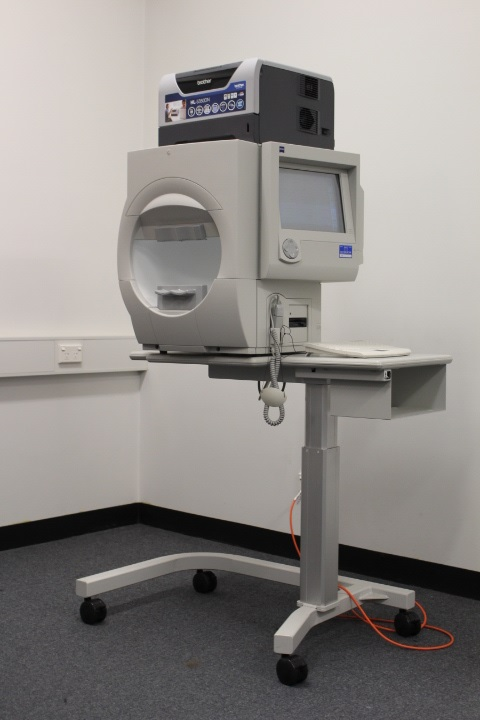
\includegraphics[width=0.5\textwidth]{hfa}
	\caption[\acl{HFA}]{\Iac{HFA} (``Humphrey VF'' by Sej licensed under \href{https://creativecommons.org/licenses/by-sa/4.0/deed.en}{CC BY-SA 4.0})}
	\label{fig:hfa}
\end{figure} 

\begin{figure}[p]
	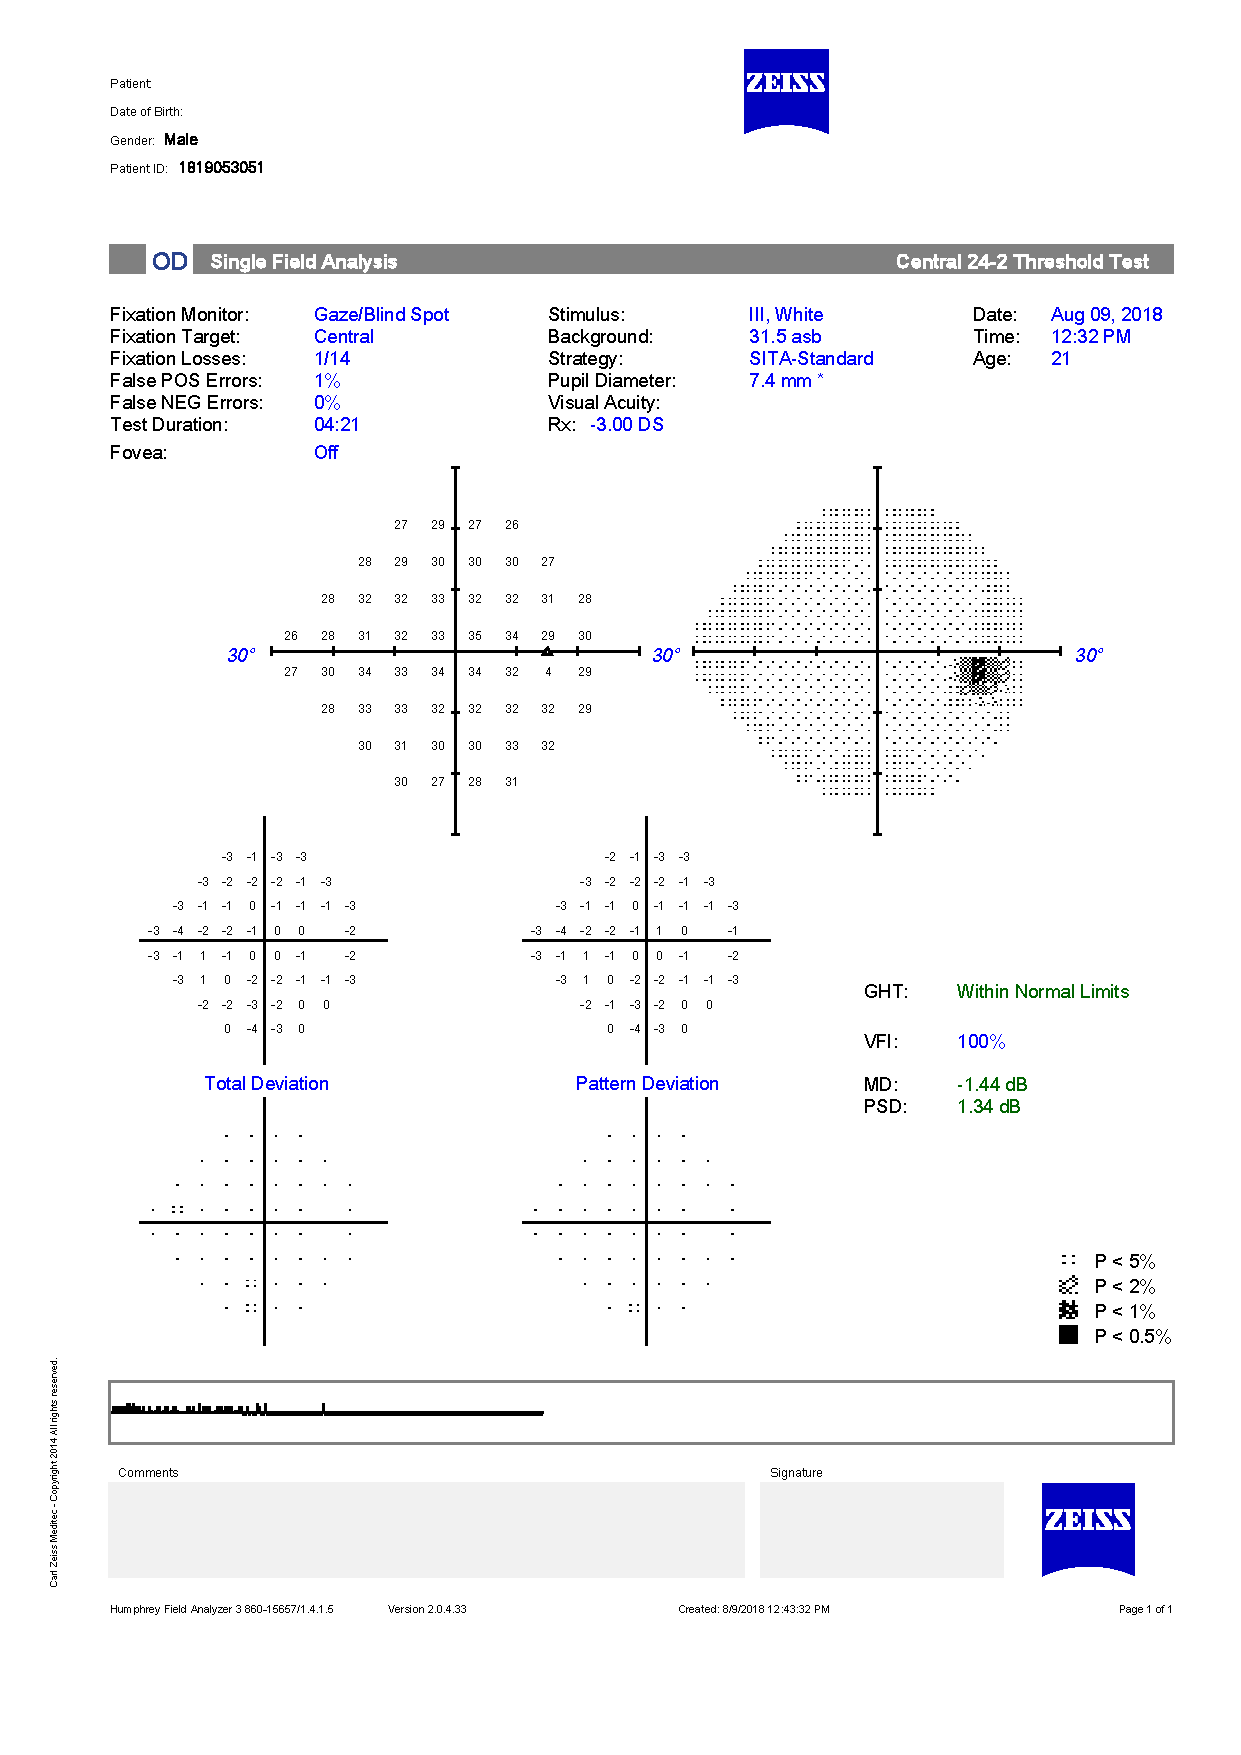
\includegraphics[width=0.9\textwidth]{report}
	\caption{Example of \iac{HFA} \acl{VF} test report}
	\label{fig:report}
\end{figure}

\begin{figure}[p]
	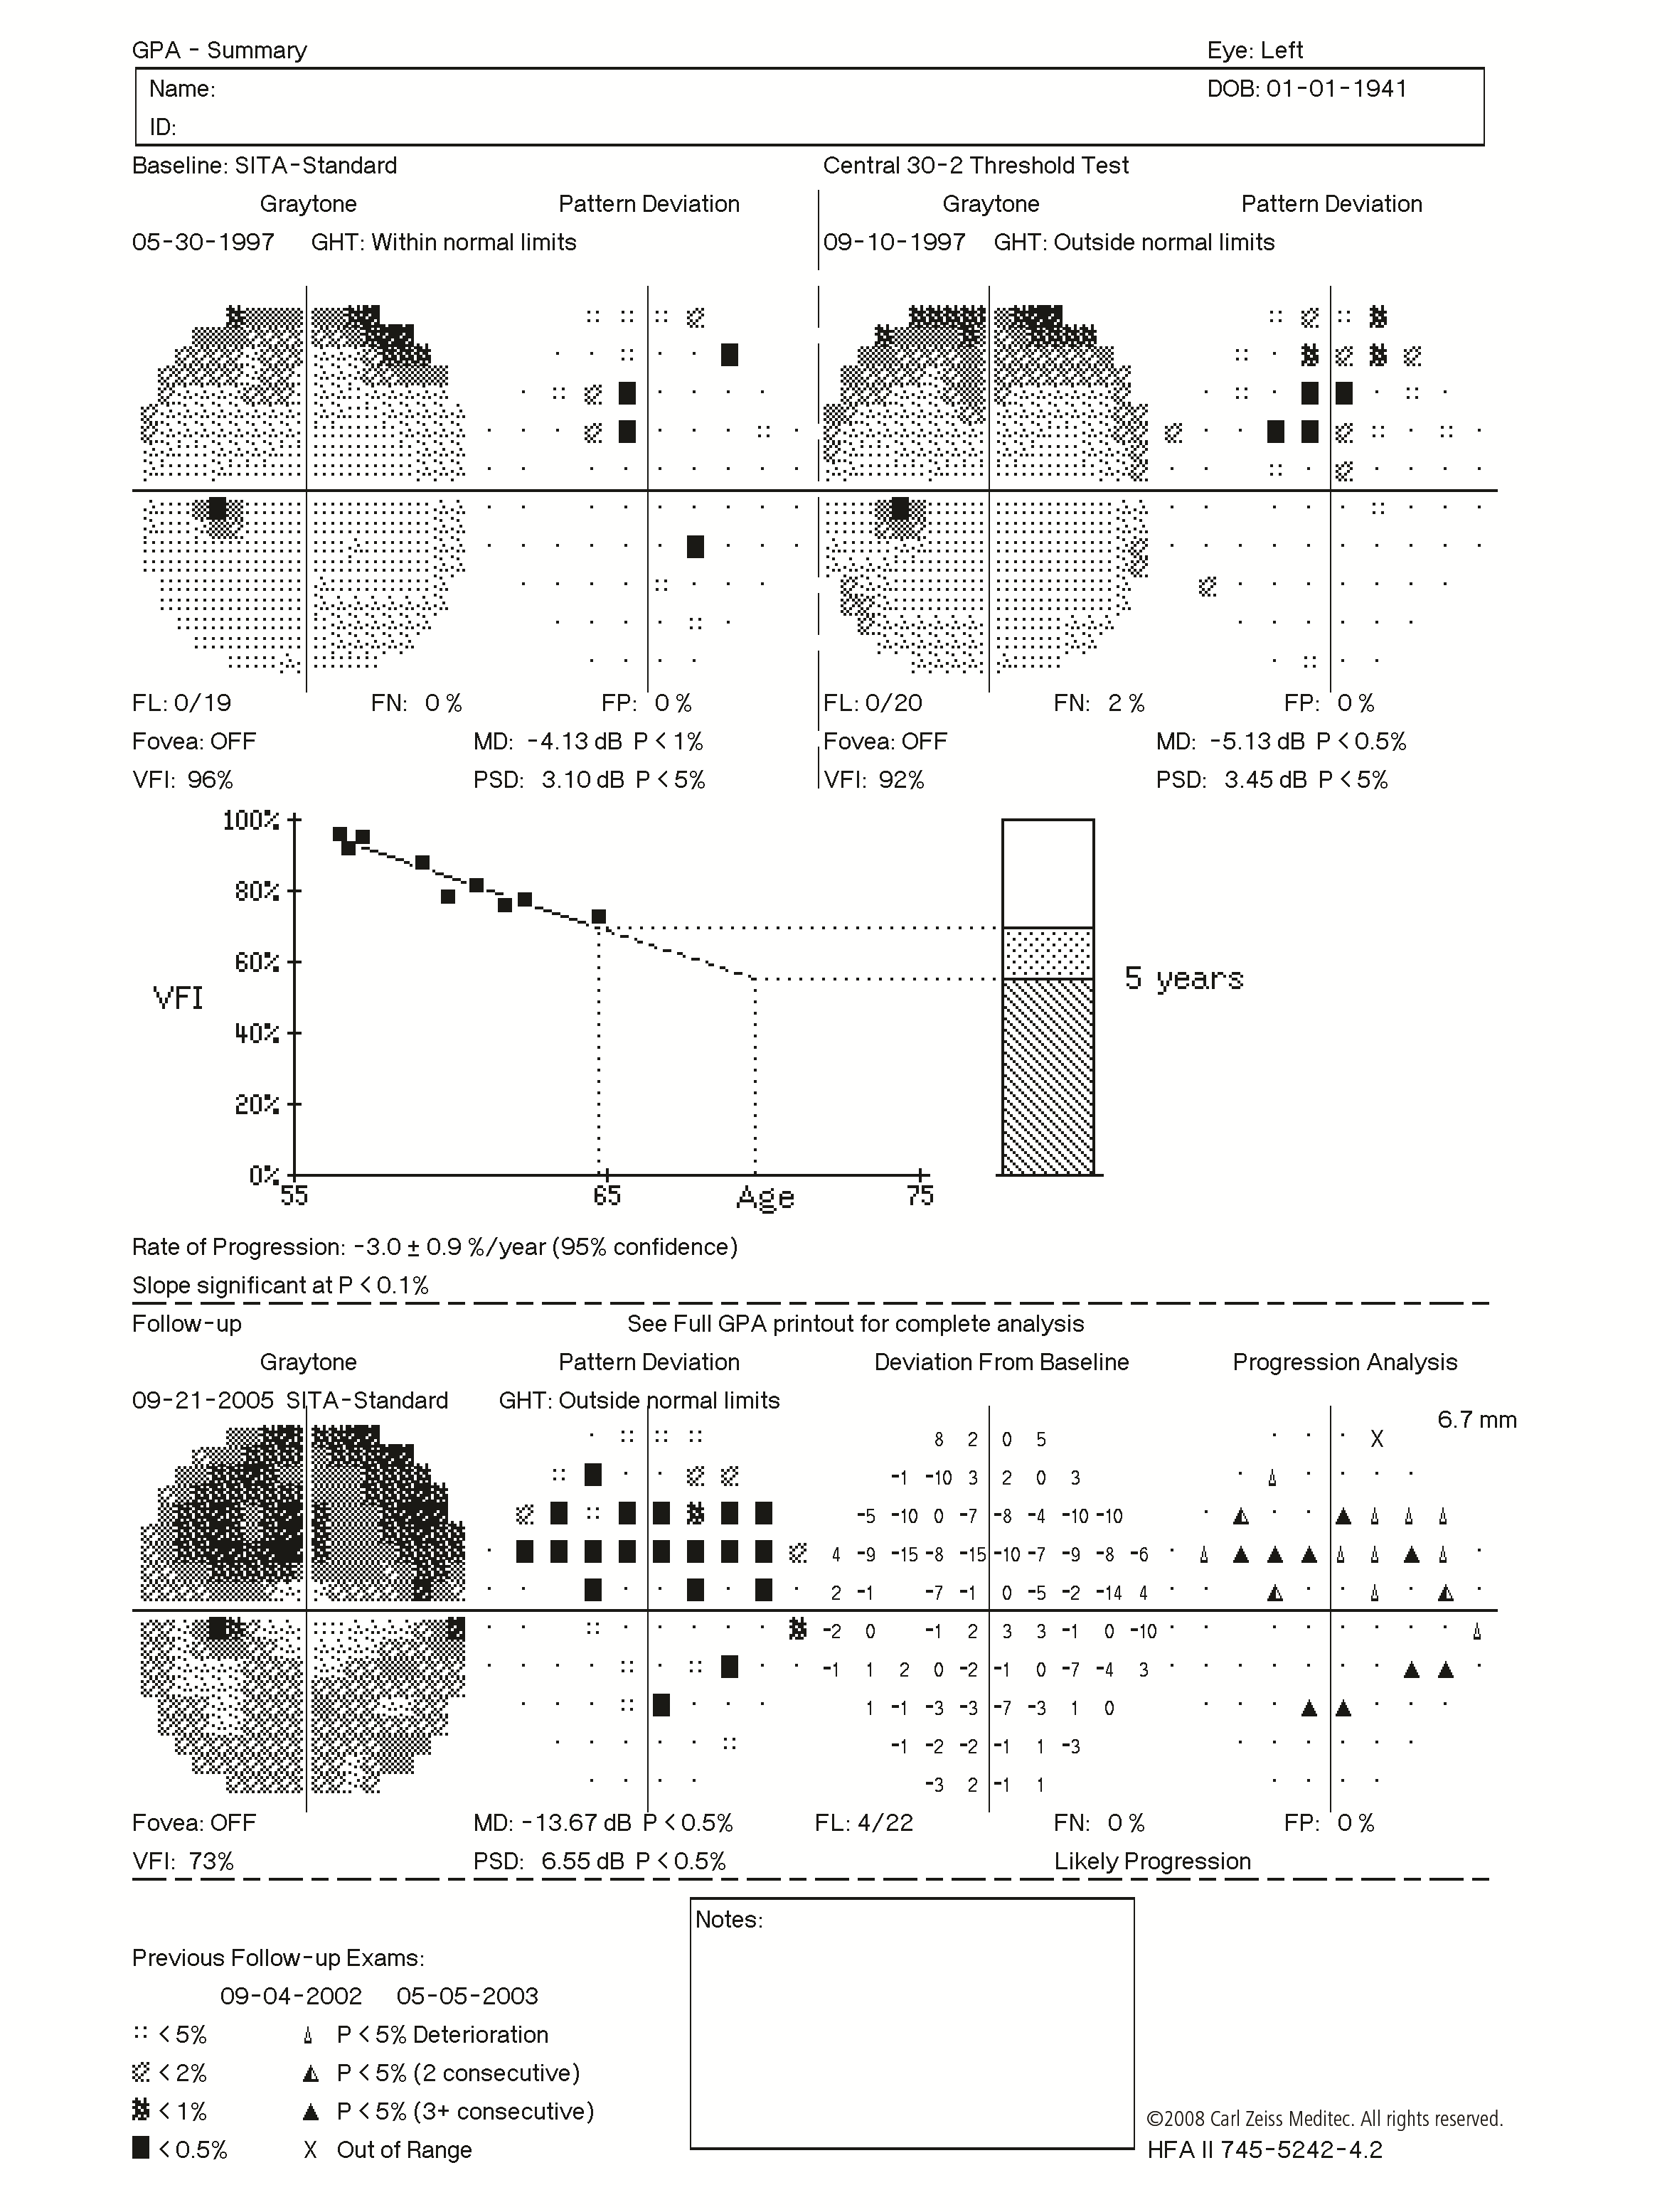
\includegraphics[width=\textwidth]{gpa}
	\caption[\Iac{HFA} progression analysis test report]{Example of \iac{HFA} progression analysis test report (Image from Carl Zeiss Meditec, Inc.)}
	\label{fig:gpa}
\end{figure}

\subsection{Single Field Analysis Metrics}

Historically Heijl et al. developed the two classic metrics for summarizing a \acl{VF}: \ac{MD} and \ac{PSD}. \cite{Heijl1987} First and foremost, to evaluate one's visual field, it is necessary to know the appropriate reference threshold ($N$) at each field location with an associated variance ($\sigma^2$). It is widely accepted that the human \ac{DLS} thresholds, in units of dB, can be modeled as a linear function of age. \cite{Heijl1987a} In general, the slope of loss of sensitivity is larger in mid-periphery than para-centrally, range from $0.5$ to $1$ dB/decade. The variance is also higher in mid-periphery than para-centrally. 

\ac{MD} is a measure of a \acl{VF}'s general mean value as compared to the reference. Mathematically, it is the mean of the difference between the measured threshold ($x$) and the reference $N$, weighted by the variance. Points with higher variance are considered less reliable and given less weight in the \ac{MD} metric; blind spots (i.e. ($15\degree$, $\pm3\degree$) are removed). MD values typically range from negative to slightly positive. Negative MD values indicate less than normal sensitivity in the entire \acl{VF} and the patient may be suspected of glaucoma and/or cataract.

\begin{equation} \label{eq:md}
\textrm{MD} =\frac{ 
\sum\limits_{i=1}^{n} \left\{
\frac{1}{\sigma_{i}^2} (x_i-N_i)
\right\} }{
\sum\limits_{i=1}^{n} 
\frac{1}{\sigma_{i}^2} 
}
\end{equation}

While the \ac{MD} is an intuitive summary metric for a \acl{VF}, it captures the general reduction in sensitivity, which is typical of cataract, but does not capture local asymmetries (variations) in the field, which is typical in a glaucomatous field. \ac{PSD} is another metric that tries to capture this asymmetry. Mathematically, it is defined as the weighted variance of the field, as defined in \cref{eq:psd}. $n$ refers to the numbers of locations, less the two blind spots, in the test pattern used for calculation (e.g. $n=54-2$ for the 24-2 pattern). \ac{PSD} is always positive, with higher value indicating a more varying field with a higher likelihood of glaucoma.

\begin{equation} \label{eq:psd}
\textrm{PSD}^2 =
	\frac{1}{n}
	\sum\limits_{i=1}^{n} 
	\sigma_{i}^2
	\times
	\frac{1}{n-1}
	\sum\limits_{i=1}^{n} 
	\frac{(x_i-N_i-\textrm{MD})^2}{\sigma_{i}^2} 
\end{equation}

Recently the new \ac{VFI} metric has become available on \ac{HFA} field analysis reports. It attempts to reduce the influence of cataract on \ac{MD} and is argued to be a better indicator for glaucoma doctors. It is reported as a percentage with $100\%$ being a perfectly healthy field and $0\%$ being a blind field. \cite{Bengtsson2008}

Another metric developed is \ac{GHT}. It combines measurement of the overall field sensitivity and differences between the top and half hemi-fields into a few hand-crafted ``if'' statements to report a field as one of the following categories for easy interpretation: \cite{Asman1992}

\begin{itemize}
	\item Abnormally high sensitivity
	\item Outside normal limits
	\item Borderline
	\item General reduction of sensitivity
	\item Within normal limits
\end{itemize}

These four metrics can be seen in figure \ref{fig:report}.

\subsection{Trend-Based Progression Analysis}

Currently, the main approach to determine glaucoma progression is a trend-based analysis by performing \ac{OLSLR} on MD. The \ac{HFA} Guided Progression Analysis reports \ac{OLSLR} on its \ac{VFI} that offers similar information. The fitted trend is typically extended five years into the future, and the slope of the line is used to classify patients into three categories (mild: $0$ to $-0.4$ dB/year, moderate: $-0.5$ to $-2$ dB/year, and severe: $<-2$ dB/year). \cite{Chauhan2008} Glaucoma specialists combine these data with additional information such as the thickness of the retinal fiber layer in the macula, \ac{IOP} and the cup-to-disk ratio to determine the optimal plan of treatment. 

\subsection{Limitations}

The current method of evaluating \acl{VF} information is limited in its robustness. For example, \ac{VFI} may remain at $100\%$ in $22\%$ patients who have MD of $-5$ dB or better. Hence early progression (up to $-5$ dB) may be missed if VFI alone is used. Moreover, based on a semi-annual follow-up schedule, at least five fields are required to produce an accurate prediction for a disease that is progressing at moderate rates (the slope of the OLSLR on MD is $-1.0$ dB/year). \cite{Chauhan2008} This means that meaningful decision about the progression of the disease cannot be made until at least two years after the initial visit. 

Last but not least, \ac{OLSLR} is a simple model chosen based on its mathematical simplicity but not upon physiology. Since glaucoma can be caused by multiple neurological pathways, it is argued that the progression trend is likely nonlinear in nature. \cite{Pathak2013} 

In short, the use of linear regression to predict \acl{VF} loss and the need for a long observation period impede timely and accurate decision making by the clinician. A better method that can provide more accurate information to the clinician in fewer \acl{VF} tests can allow more effective intervention for glaucoma patients in the disease's early stages. This is the primary motivation for the alternative models reviewed below and for the current work.

\section{Literature Review: Alternative Progression Models}

This section will review alternatives to the \ac{OLSLR} on MD model for \acl{VF} progression prediction. 

\subsection{Statistical Models}

A complement to trend-based analysis is event-based analysis. A popular implementation is the Glaucoma Progression Analysis (GPA) since it is provided by the \ac{HFA}. Instead of fitting a trend on a global index, the progression of each point in the field with respect to a baseline measurement is considered. On average, this method is found to have low false-positive rate. However, this is dependent upon achieving a good baseline and does not work for patients with severe \acl{VF} loss. \cite{Aref2017}

Other non-linear models suggest fitting an exponential model to the \acl{VF} indices. For example, Pathak et al. argued that an exponential model is better supported by recent knowledge of structure-function relationship than a linear model. \cite{Pathak2013} They demonstrated that a linear mixed-effect (LME) approach with an exponential model provided significantly better prediction of glaucoma progression than linear models. However, it is also pointed out that even though the LME approach has better results than the \ac{OLSLR} it still cannot capture the full extent of glaucomatous \acl{VF} change.

Other innovative approaches to the glaucoma progression problem in the literature include:

\begin{itemize}
	\item Point-wise linear regression (PLR): Developed for improving early detection, PLR combines event-based and trend-based analysis \cite{Nouri-Mahdavi2005}. 
	\item Analysis with Non-Stationary Weibull Error Regression and Spatial Enhancement (ANSWERS): Using spatial correlation between points and incorporating non-stationary variability; progression detection was found to be better especially in short time series \cite{Zhu2015}.
	\item Spatially filtering \acl{VF} data before PLR analysis: By applying a spatial filter that incorporates physiological relationships between measured contrast sensitivities at test points within the visual field, the specificity of the PLR method is not affected but the sensitivity of detecting the rate of progression is improved \cite{Strouthidis}.
\end{itemize}

\subsection{Machine Learning Models}

The above methods use different approaches to improve the prediction of glaucoma progression and demonstrate the complexity of the prediction task. This is not surprising due to the complex nature of the disease. A natural step forward involves leveraging the power of modern \ac{ML} techniques to integrate features such as non-linear trends, correlation between \acl{VF} test locations, field patterns, etc. into a single model.
 
Existing studies have demonstrated the usefulness of \ac{ML} in glaucoma care. For example, Asaoka et al. compared the performance of traditional ML classifiers with that of a deep feed-forward neural network (FNN) in diagnosing preperimetric glaucoma with visual field data \cite{Asaoka2016}. Their FNN model performed significantly better than other methods. In another study, Yousefi et al. applied clustering algorithms to extract visual field patterns as features, then adapted the traditional linear regression algorithm to model the features to generate the predictions \cite{Yousefi2018}. The \ac{ML}-based index for the detection of glaucoma progression outperformed current methods. 

However, these studies either did not directly address the problem of predicting \acl{VF} progression or only used traditional \ac{ML} methods for initial feature extraction. In a recent study that fully utilized the power of \ac{ML} for the prediction task, Wen et al. \cite{Wen2018} used deep learning network to predict future visual field given the measurements of a single current \acl{VF}. Their deep learning network demonstrated amazing capability to generate prediction for future visual fields for up to $5.5$ years with a correlation of $0.92$ between the predicted \ac{MD} and actual future \ac{MD} (average difference of $0.41$ dB). Their results suggest the tremendous potential of this research area. 

Another benefit of using an \ac{ML} model is the ability to use visual field data (i.e. functional indication of \acl{VF} integrity) and \ac{OCT} data (i.e. structural indication for the integrity of the retina) at the same time. It is known that by utilizing both \acl{VF} and \ac{OCT} data the sensitivity of glaucoma detection can be improved \cite{Shah2006}, \cite{Lu2008}. Multivariate models including both \acl{VF} and \ac{OCT} have also been shown to be successful \cite{Mwanza2013}. However, there is limited research on combining \acl{VF} and \ac{OCT} features through a \ac{ML} model. A limited attempt to explore this idea by Silva et al. did not produce better results than those obtained by \acl{VF} only parameters \cite{Silva2013}. 

In our study we plan to use \ac{ML} models that combine \acl{VF} and \ac{OCT} data for prediction of disease progression.  Specifically, we will use a deep \ac{RL} approach to the glaucoma progression problem. Deep RL has gained attention lately due to its use in solving seemingly impossible problems. The most well-known example is solving the ancient Go game, which is considered to be orders of magnitude more difficult than chess and other board games \cite{Silver2016}. \ac{RL} has also been used in the context of healthcare for discovering optimal, individualized treatment strategies for lung cancer \cite{Zhao2009}\cite{Zhao2011}, HIV \cite{Ernst2006} and neurological disorders \cite{Shortreed2011}. To the best of our knowledge this will be the first study to use \ac{RL} to predict glaucoma progression. 



\chapter{Progress to Date}

\section{Rotterdam Longitudinal Glaucomatous \ac{VF} Dataset}

The Longitudinal Glaucomatous Visual Field data from Rotterdam Ophthalmic Data Repository \cite{Bryan2013} consists of data from $139$ patients' $278$ eyes. A total of $4863$ 24-2 test results with MD are available. On average each eye has $17.5$ fields available with mean follow-up time of $9.2$ years. $270$ $(97.1\%)$ eyes have at least $14$ fields with a minimum of $7.6$ years of follow-up. The mean and median follow-up interval between tests is $203$ and $189$ days; the standard deviation of follow-up time is $72.3$ days. $346$ $(7.5\%)$ of follow-ups had an interval of more than $270$ days. 

\subsection{Data Characteristics}

To investigate the composition of healthy versus glaucomatous patients the dataset, the characteristic of MD values in the dataset is investigated. In figure \ref{fig:mean_md_hist} the distribution of average MD value calculated from all tests administers on an eye for each of the $278$ eyes is shown. The mean and median of the distribution are $-8.9$ and $-6.8$ dB respectively. The data set contains mostly eyes with mild to moderate reduced MD values ($75\%$ of eyes have average MD $>-13.2$ dB).

\begin{figure}[h]
	\centering
	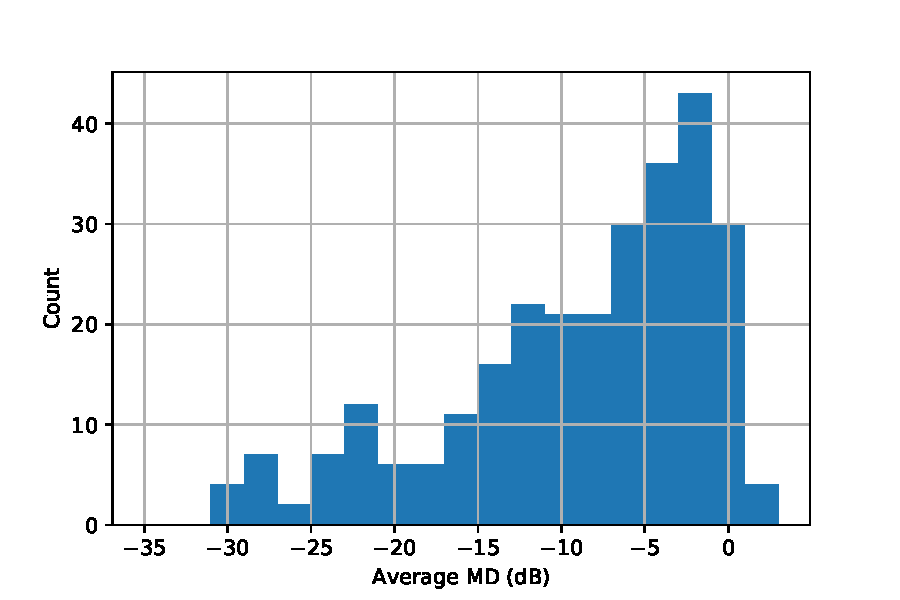
\includegraphics[width=0.6\textwidth]{mean_md_hist}	\caption{Distribution of eyes' average MD values within the Rotterdam dataset ($n=278$)}
	\label{fig:mean_md_hist}
\end{figure}
%
%\begin{figure}[h]
%	\centering
%	\begin{subfigure}[b]{0.45\textwidth}
%		\centering
%		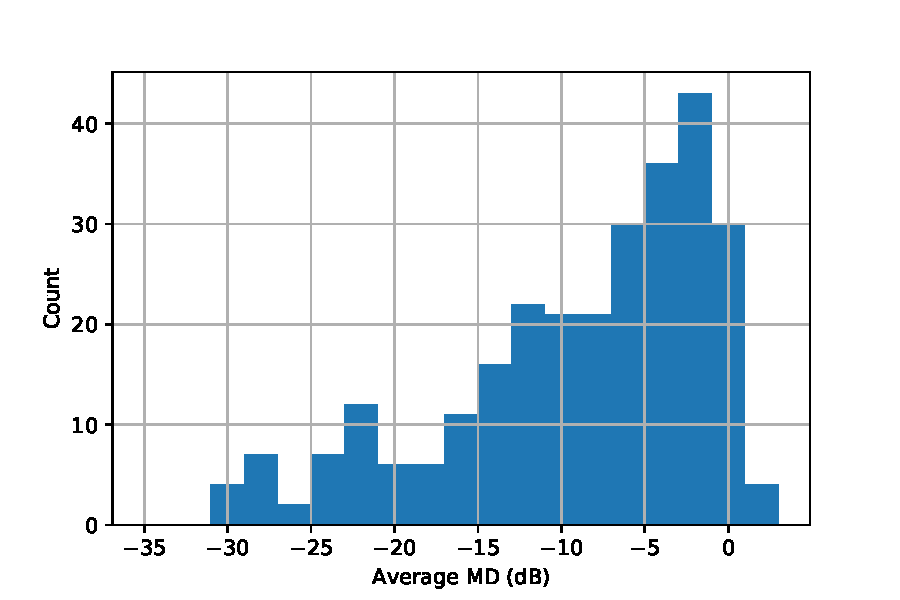
\includegraphics[width=\textwidth]{mean_md_hist}
%		\caption{}
%		\label{fig:mean_md_hist}
%	\end{subfigure}
%	\hfill
%	\begin{subfigure}[b]{0.45\textwidth}
%		\centering
%		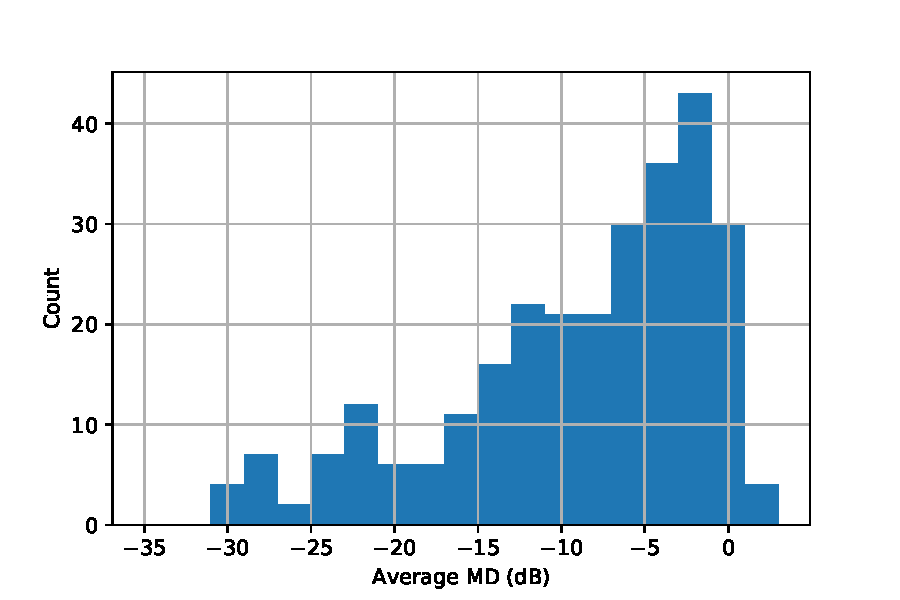
\includegraphics[width=\textwidth]{mean_md_hist}
%		\caption{}
%		\label{fig:three sin x}
%	\end{subfigure}
%	\caption{(a) Distribution of MD values within the patient dataset}
%	\label{fig:study_site}
%\end{figure}
%
%
%
%


\chapter{Learning Methods}

This chapter provides a framing of the visual field progression prediction tasks introduced before as learning problems, and introduces the learning algorithm architectures to be evaluated against the available data set. 

\section{The Learning Task}

\subsection{Formulation and Normalization}

Given the information in the Rotterdam dataset, we can write each patient visit as one feature vector as follows:

\begin{equation}
v^{(i)} = \begin{bmatrix}
\textrm{VF}^{(i)}_1 & 
\textrm{VF}^{(i)}_2 & 
\cdots & 
\textrm{VF}^{(i)}_{54} & 
\textrm{MD}^{(i)} & 
\textrm{IOP}^{(i)} & 
t^{(i)}
\end{bmatrix}
\in \mathbb{R}^{57}
\end{equation}

where $t^{(n)}$ is the time of the visit, and $\textrm{VF}^{(i)}_j$ is the \ac{DLS} for the $j$-th point in the visual field. By convention of the visual field analysis tools developed by Marin-Franch et al. \cite{Marin-Franch2013}, all fields of the left (OS) eye are flipped horizontally (unmodified vertically) to match with the coordinates of the right eye, and then each visual field location is index from left to right, then top to bottom, in the same way as the reading direction in English. Each of the vector component is normalized in the range shown in \cref{tab:norm}.

\begin{table}[h]
\centering
\caption{Feature range normalization with appropriate physiological ranges}
\begin{tabular}{@{}lrrrc@{}}
\toprule
 & \multicolumn{3}{c}{Normalization Range} & \\
\cmidrule{2-4}
Feature & Lower (0) & Upper (1) & Unit & Comments \\ 
\midrule
VF & 0 & 40 & dB &  \\
MD & 0 & 40 & dB & Negative sign preserved \\
IOP & 0 & 20 & mmHg &  \\
Age ($t$) & 50 & 80 & years &  \\ 
\bottomrule
\end{tabular}
\label{tab:norm}
\end{table}

For three input fields, we can concatenate the three visits and write the entire input vector as: 

\begin{equation}
x^{(n)} = \begin{bmatrix}
v^{(i)} & v^{(i+1)} & v^{(i+1)}
\end{bmatrix}
\in \mathbb{R}^{171}
\end{equation}

\subsection{Learning Dataset Generation}

The entire dataset can be put into matrix form, where the input is:

\begin{equation}
\mathbf{X} = \begin{bmatrix}
x^{(1)} \\
x^{(2)} \\
\vdots \\
x^{(N)} \\
\end{bmatrix}
\in \mathbb{R}^{N\times 161}
\end{equation}

and the output field prediction is simply the \ac{DLS} at each location:

\begin{equation}
\mathbf{Y} = \begin{bmatrix}
Y^{(1)} \\
Y^{(2)} \\
\vdots \\
Y^{(N)} \\
\end{bmatrix}
= \begin{bmatrix}
\textrm{VF}_1^{(1)} & \textrm{VF}_2^{(1)} & \cdots & \textrm{VF}_{54}^{(1)} \\
\textrm{VF}_1^{(2)} & \textrm{VF}_2^{(2)} & \cdots & \textrm{VF}_{54}^{(2)} \\
& \vdots & & \\
\textrm{VF}_1^{(N)} & \textrm{VF}_2^{(N)} & \cdots & \textrm{VF}_{54}^{(N)}
\end{bmatrix}
\in \mathbb{R}^{N\times 54}
\end{equation}

Since it is fairly standard---and also the case in the Rotterdam dataset as shown before---that glaucoma patients are followed up on an interval of 6 months, the training examples are generated such that

\begin{equation} \label{eq:train-criterion-1}
\Delta t = 183~\textrm{days} \approx (t_{v^{(i+1)}} - t_{v^{(i)}}) \approx (t_{v^{(i+2)}} - t_{v^{(i+1)}})
\end{equation}

and the output field is $K$ fields (approximately $0.5K$ years) after the last input field:

\begin{equation} \label{eq:train-criterion-2}
t_{v^{(Y)}} - t_{v^{(i+1)}} \approx 183K~\textrm{days}
\end{equation}

Learning sets in the Rotterdam dataset that satisfy \cref{eq:train-criterion-1,,eq:train-criterion-2} for all $K\in[1, 10]$ are generated.

\subsection{Error Definition}

The \ac{MAE} error for the whole field is defined as:

\begin{equation}
L(\hat{y}, y) = \textrm{MAE}_{\vf} \triangleq 
\frac{1}{54N} \sum_{n=1}^N \sum_{j=1}^{54} \left|  \widehat{\vf}_j^{(n)} - {\vf}_j^{(n)}  \right|
\end{equation}

The \ac{MAE} error for \ac{MD} is defined as:

\begin{equation} \label{eq:mae-md}
%\textrm{MAE}_{\md} \triangleq
\frac{1}{N} \sum_{n=1}^N \left|  \widehat{\md}^{(n)} - {\md}^{(n)}  \right|
\end{equation}

The calculation of \ac{MD} was introduced as \cref{eq:md}, which requires 1) age-adjusted baseline \ac{DLS} values and 2) variance at each location of the field (i.e. weights when averaging the deviation values). Since the target \ac{MD} values in the Rotterdam database are provided presumably from \ac{HFA}'s database that are not publicly available, one can modify \cref{eq:mae-md} by substituting in \cref{eq:md}:

\begin{align}
\textrm{MAE}_{\md} &=
\frac{1}{N} \sum_{n=1}^N \left| 
\sum_{j=1}^{54} w_j \left( \widehat{\vf}_j^{(n)} - N_j \right) - 
\sum_{j=1}^{54} w_j \left( {\vf}_j^{(n)} - N_j \right)  \right| \\
&=
\frac{1}{N} \sum_{n=1}^N \left| 
\sum_{j=1}^{54} w_j \left( \widehat{\vf}_j^{(n)} - \vf_j^{(n)} \right) \right|
\end{align}

where $N_j$ is the age-adjusted population normal value at the $j$-th visual field point, and 

\begin{equation}
w_j=\frac{ \frac{1}{\sigma_{j}^2} }{
	\sum\limits_{i=1}^{n} 
	\frac{1}{\sigma_{i}^2} 
}
\end{equation}

. This expression is only dependent upon the weights used in calculating \ac{MD}, since the age-adjusted baseline cancels out. The weights are available from Heijl et al. \cite{Heijl1987} or Marin-Franch et al. \cite{Marin-Franch2013}

\subsection{Evaluation Procedure}

$70\%$ of the data is used for training, $15\%$ is used for validation and used to fine tune the hyper-parameters of the model. Then, the hyper-parameters are set and 5- or 10-fold cross validation is performed to report model performance. 

\section{Models}

This section describes a range of simple to complex learning models that are proposed for evaluation for the learning task. Simpler models might be more robust to noise in the visual field dataset and generalize better for the limited data available, while a complex model might extract more powerful visual field and patient features from the data at the peril of over-fitting. 

\subsection{Ridge Regression}

Ridge regression is a $L_2$-regularized linear regression\footnotemark that aims to minimize the combination of the sum squared cost and the $L_2$ norm of the weight parameters. By weighting on the model parameters, one hopes to yield a simpler model that is fit less toward specific trends in the training set and generalizes better. The model prediction is: 

\footnotetext{In this document the term ``linear regression'' is intentionally avoided to avoid confusion with the simple linear extrapolation method by extrapolating each variable with a linear fit over time, which is often called the \ac{OLSLR} method.}

\begin{equation}
\hat{\mathbf{Y}} = \mathbf{X}_1\mathbf{W}
\end{equation}

where $\mathbf{X}_1\triangleq\begin{bmatrix}\mathbf{1} & \mathbf{X} \end{bmatrix}$ includes the bias feature. The objective is to minimize the regularized sums squared cost:

\begin{equation}
\mathbf{W} \leftarrow \arg \min_{\mathbf{W}} ||\hat{\mathbf{Y}} - \mathbf{Y}||^2_2 + \lambda ||\mathbf{W}||^2_2
\end{equation}

This has the closed form solution, which is directly implemented:

\begin{equation}
\mathbf{W} = \left(
\mathbf{X}_1^T \mathbf{X}_1 + \lambda I
\right)^{-1}
\mathbf{X}_1^T \mathbf{Y}
\end{equation}

\subsection{Huber Regression}

The Huber linear regressor uses a cost metric that is more robust to outliers, with the following definition:

\begin{equation}
L(\hat{y}_j, y_j) = \left\{\begin{array}{lr}
\frac{1}{2}(\hat{y}_j - y_j)^2, & |\hat{y}_j - y_j| \leq \delta\\
\delta|\hat{y}_j - y_j| - \frac{1}{2} \delta^2, & |\hat{y}_j - y_j| > \delta\\
\end{array}
\right.
\end{equation}

Intuitively, for points close to the target, a squared cost is used, while for points further away than a threshold (e.g. outliers), a linear cost is used. Therefore it is also known as a robust regressor. One may hope that it may be better at rejecting noise from visual field recordings. 

One Huber regressor is needed for each output dimension, so essentially 54 regressors are fit with the same input. Implementation wise, this is done by chaining \verb|HuberRegressor| into \verb|MultiOutputRegressor| using the Scikit-learn library. \cite{scikit-learn} There is no closed-form solution for Huber regression so an iterative solution is found. 

\subsection{Multi-Layer Perceptron}

The \ac{MLP} neural network model takes the 171 features as input and outputs 54 \ac{DLS} values. Considering the high dimensionality of the output, a standard three-layer (two hidden layers) network is investigated with number of neural units being the hyperparameter. $L_2$ regularization is applied to all weights. ReLU is used as the activation function at all layers except the output layer. The model is implemented in Tensorflow. \cite{tensorflow} The whole field \ac{MAE} loss is used as the objective function. The weights are optimized iteratively with the Adam Optimizer using batch size of 32.

\subsection{Convolutional Neural Network}

\ac{CNN} is a type of neural network architecture that, thanks to the tremendous improvement in computational power recently, has shown tremendous performance in automatically learning to extract image features instead of requiring hand-crated features detection algorithms. Each visual field can be seen as an $8\times9$ image. This relatively low dimensionality, compared to the inputs to typical image recognitions tasks in which \acp{CNN} are applied, may leave limited room of improvement in the performance of \ac{CNN} over a simpler flat architecture such as \iac{MLP}. However, spatial patterns in the visual field are have been known to important to glaucoma diagnosis and progression, and \ac{CNN} is an architecture that is known to be able to extract such spatial information. 

\begin{figure}[p]
	\centering
	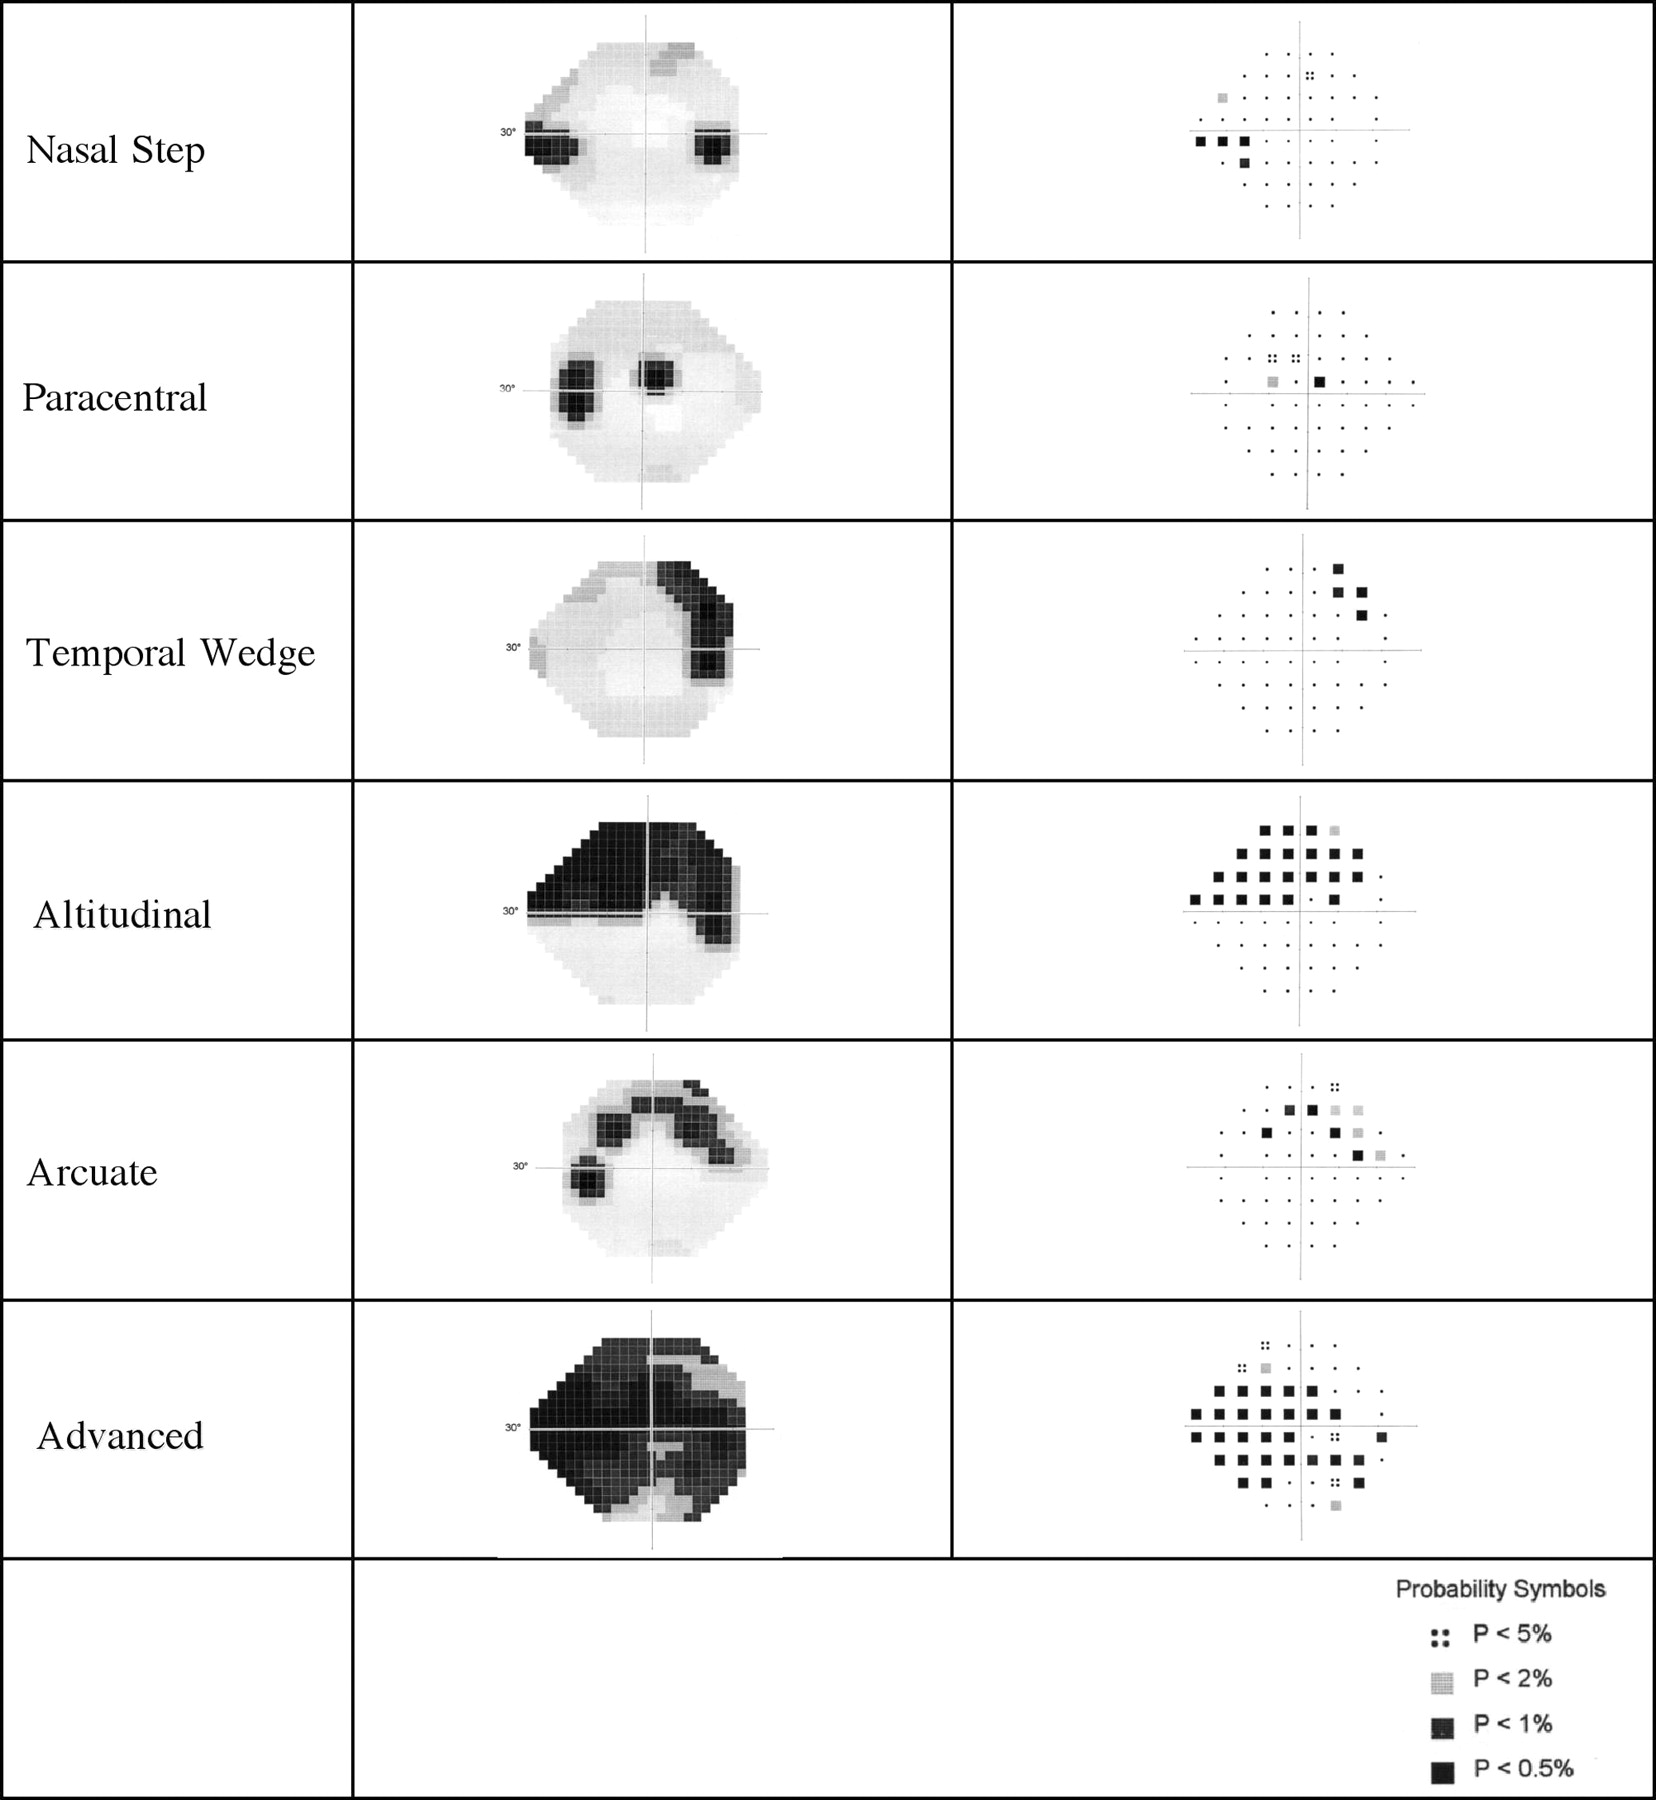
\includegraphics[width=\textwidth]{sample2004pattern}
	\caption[Examples of typical patterns of glaucomatous visual field loss]{Examples of typical patterns of glaucomatous visual field loss that are known to be physiologically and clinically important for diagnosis and prediction. Such evidence is the motivation behind employing a \ac{CNN} achitecture that is likely to preserve and extract useful spatial information in the visual field. (Figure from Sample et al. \cite{Sample2004})}
\end{figure}

A typical \ac{CNN} architecture is implemented. Specifically, this \ac{CNN} consists of:

\begin{enumerate}
\item Input layer: Input is three visual field ``images'' stacked ($8\times9\times3$). Locations outside the 24-2 examination area are replaced with zeros. 
\item First convolutional layer with $3\times3$ kernel, stride length $1$. Output is passed through ReLU activation and batch normalization. 
\item Max pool layer with pool size and stride length of $2$. 
\item Second convolutional layer with $3\times3$ kernel, stride length $1$. Output is passed through ReLU activation and batch normalization, then flattened. 
\item Additional features (i.e. MD, IOP, and Age) are concatenated to the vector. 
\item First fully connected hidden layer. Output is passed through ReLU activation and a dropout layer. 
\item Second fully connected hidden layer. 
\item Output layer. ($d=54$)
\end{enumerate}

The modeled is trained using Adam Optimizer to minimize the $L_2$ regularized \ac{MAE} loss, and implemented with Tensorflow. \cite{tensorflow} The number of channels in the \ac{CNN}, neural units in the fully-connected layer, and regularization are fine-tuned as hyperparameters. 

\subsection{Deep CNN+LSTM Network}

The final proposed framework involves adding the \ac{LSTM} network to the \ac{CNN} network. The \ac{LSTM} module is a type of \ac{RNN}. Its recurrent nature allows modeling of sequential data; in the case of the current prediction task, it is used to model the sequential visual field inputs at different time points. 

The \ac{LSTM} network also has the benefit of only needing one network to predict multiple outputs in the future due to its recurrent nature. Because of this, the training dataset used to train this network is slightly different from networks above. When training this network, it is necessary to generate a sequence of all fields $i=0, 1, 2, (2+1), (2+2), \dots, (2+K)$ where $K$ is the maximum number of fields in the future that is desired to be predicted. At test time, the model takes fields $i=0, 1, 2$ as input, and outputs all field predictions at $i=(2+1), (2+2), \dots, (2+K)$. $K=5$ and $K=10$ are tested, where $K=5$ is expected to include more training examples. 

The detailed procedure of this network is shown as \cref{algo:CNNLSTM} in \cref{chapter:code}. The network is implemented using the PyTorch framework. \cite{paszke2017automatic} 




\chapter{Results and Discussion}

\section{Model Parameters}

Using the $70\%$ training set, $15\%$ validation set, and $15\%$ testing set, the hyperparameters chosen for each learning model is shown in \cref{tab:hyperparam}.

\begin{table}[h]
	\centering
	\caption{Final hyperparameters for learning models}
	\label{tab:hyperparam}
	\begin{tabular}{@{}ll}
		\toprule
		Model                & Parameters                                                                                    \\ \midrule
		Ridge Regression     & $\lambda=10$                                                                                  \\ \midrule
		Huber Regression     & $\epsilon = 1.0$                                                                              \\
		                     & $\alpha=0.001$                                                                                \\
		                     & ($\epsilon$ and $\alpha$ are specific to the Scikit-learn implementation \cite{scikit-learn}) \\\midrule
		\acs{MLP}            & Size of first hidden layer: $200$                                                             \\
		                     & Size of second hidden layer: $150$                                                            \\ \midrule
		\acs{CNN}            & $L_2$ Regularization: $\lambda=0.8$                                                           \\
		                     & Convolution layers depth: $(128, 256)$                                                        \\
		                     & Fully connected layers size: $(512, 256)$                                                     \\ \midrule
		\acs{CNN}+\acs{LSTM} & $L_2$ Regularization: $\lambda=0.0001$                                                             \\
		                     & \acs{LSTM} hidden state size: 4096                                                            \\
		                     & Convolution block size for three convolution blocks: $(64, 128, 256)$                         \\ \bottomrule
	\end{tabular}
\end{table}

\section{Cross Validation Results}


\begin{figure}[p]
\begin{minipage}{\textwidth}
	\centering
	\begin{subfigure}[b]{\textwidth}
		\centering
		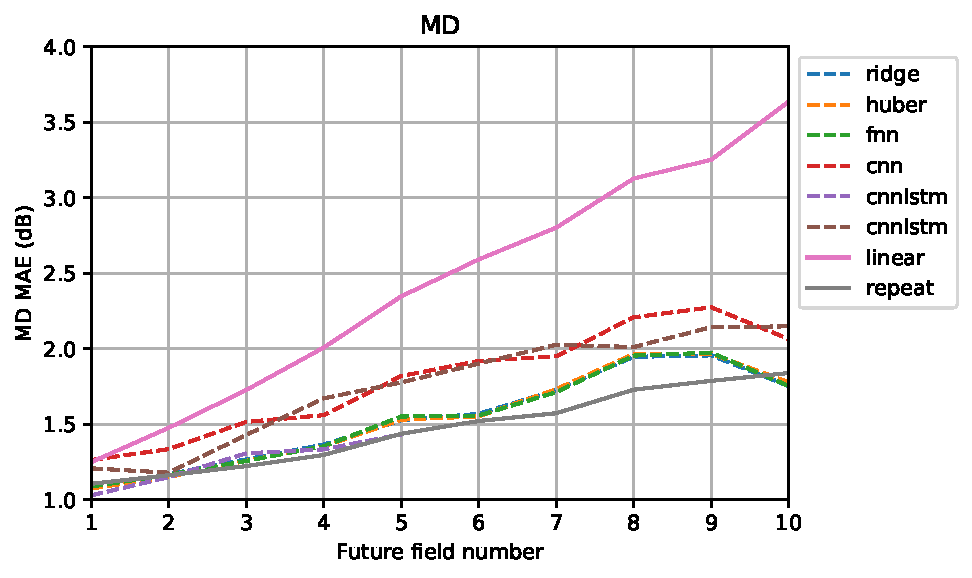
\includegraphics[width=0.8\textwidth]{ml_md.pdf}
		\caption{}
	\end{subfigure}
	\hfill
	\begin{subfigure}[b]{\textwidth}
		\centering
		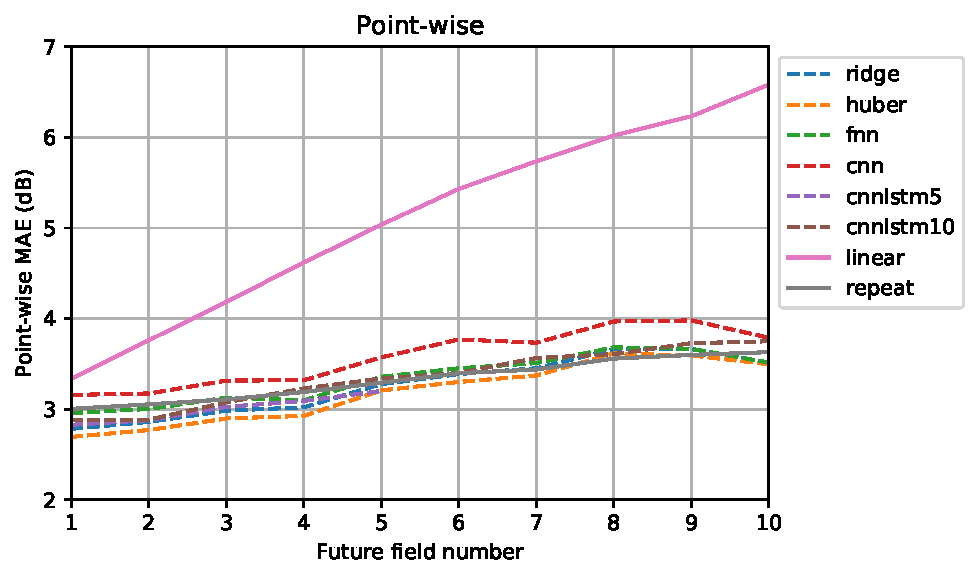
\includegraphics[width=0.8\textwidth]{ml_vf.pdf}
		\caption{}
	\end{subfigure}
	\caption[\acs{MD} and point-wise field prediction results for learning algorithms]{\acs{MD} and point-wise field prediction results for learning algorithms with 3 inputs, compared to the linear extrapolator and repeating the last observed value ``repreat''. There is no significant difference between the learning methods, and due to the dataset containing mostly stable patients, there is no significant difference between the learning methods and ``repeat''. However, all methods performed better than the linear extrapolation methods. \footnote{In an earlier version of this figure, it was shown that the CNN+LSTM model performed slightly better than other learning methods. This has been corrected in this latest batch of experiments.}}
	\label{fig:ml_fig}
\end{minipage}
\end{figure}

\begin{table}[t]
	\centering
	\caption{Learning algorithm performance for the 5-th and 10-th prediction}
	(25\%/50\%/75\% are the 25-th percentile/median/75-th percentile respectively)
	\label{tab:ml_tab}
	
	\hspace*{-1.5cm}
	\begin{tabular}{@{}llllllllll@{}}
		\toprule
		Prediction &      &   \multicolumn{6}{c}{Learning Algorithm} &  \multicolumn{2}{c}{Extrapolation}  \\
		\cmidrule(lr){3-8} \cmidrule(lr){9-10}
		\acs{MAE} (dB) &      & Ridge & Huber & \acs{MLP}  & \acs{CNN}  & CNN+LSTM5 & CNN+LSTM10 & Linear & Repeat \\ \midrule
		& mean & 1.53  & 1.53  & 1.55 & 1.82 & 1.43     & 1.78      & 2.35   & 1.44   \\
		MD, & std  & 1.7   & 1.73  & 1.76 & 1.83 & 1.44     & 1.63      & 2.75   & 1.59   \\
		5-th& 25\% & 0.45  & 0.45  & 0.44 & 0.59 & 0.49     & 0.59      & 0.64   & 0.43   \\
		& 50\% & 1.05  & 1.02  & 1.04 & 1.3  & 1.03     & 1.44      & 1.41   & 0.99   \\
		& 75\% & 1.93  & 1.93  & 1.97 & 2.5  & 1.93     & 2.3       & 2.95   & 1.85   \\
		\midrule
		& mean & 1.75  & 1.78  & 1.75 & 2.06 &          & 2.15      & 3.64   & 1.84   \\
		MD, & std  & 1.75  & 1.76  & 1.78 & 2.01 &          & 2.16      & 4.28   & 2.17   \\
		10-th & 25\% & 0.57  & 0.6   & 0.57 & 0.64 &          & 0.65      & 0.81   & 0.51   \\
		& 50\% & 1.27  & 1.27  & 1.23 & 1.45 &          & 1.47      & 1.91   & 1.18   \\
		& 75\% & 2.32  & 2.29  & 2.24 & 2.8  &          & 2.79      & 4.94   & 2.3    \\
		\midrule
		& mean & 3.28  & 3.21  & 3.36 & 3.57 & 3.2      & 3.34      & 5.04   & 3.29   \\
		Point-wise, & std  & 3.55  & 3.63  & 3.85 & 4.08 & 3.69     & 3.87      & 5.85   & 4.18   \\
		5-th& 25\% & 0.95  & 0.89  & 0.88 & 0.94 & 1        & 1         & 1      & 1      \\
		& 50\% & 2.14  & 2.02  & 2.04 & 2.21 & 1.91     & 1.94      & 3      & 2      \\
		& 75\% & 4.25  & 4.1   & 4.27 & 4.53 & 4        & 4.1       & 7      & 4      \\
		\midrule
		& mean & 3.51  & 3.5   & 3.51 & 3.79 &          & 3.75      & 6.58   & 3.63   \\
		Point-wise, & std  & 3.58  & 3.74  & 3.86 & 4.16 &          & 4.33      & 7.39   & 4.6    \\
		10-th& 25\% & 1.11  & 1.05  & 1    & 1.03 &          & 1         & 1      & 1      \\
		& 50\% & 2.42  & 2.34  & 2.24 & 2.41 &          & 2.21      & 4      & 2      \\
		& 75\% & 4.61  & 4.54  & 4.54 & 4.94 &          & 4.64      & 10     & 5      \\ \bottomrule
	\end{tabular}
\end{table}

5-fold cross validation is performed on the learning models with hyperparameters listed in \cref{tab:hyperparam}. The same cross-validation set is used for ridge regression, Huber regression, \ac{MLP}, and \ac{CNN}. A different sequence is used for the \acs{CNN}+\acs{LSTM} model due to the recurrent structure of the \ac{LSTM} module; sequences extending to 5 and 10 fields into the future are investigated for \acs{CNN}+\acs{LSTM}. These results are compared to the linear extrapolation method and the repeat-last-value (``repreat'') method, which were described in \cref{sec:extrapresult}. A detailed comparison of the performance of different methods at predicting 5 and 10 fields in the future is tabulated in \cref{tab:ml_tab}.

Using the Rotterdam dataset, there is no significant difference between the learning algorithms evaluated for both the \ac{MD} prediction task \ac{MAE} and the point-wise whole field task \ac{MAE}. Furthermore, there is no significant difference between the learning and repeat method for both tasks. The linear extrapolation method performed much worse than all other methods in terms of mean, median, and 75-th percentile error, but the 25-th percentile error is similar. 

Within each method, the error increases as one extends the prediction further into the future. In addition, the \ac{MD} prediction \ac{MAE} is in general approximately one half that of the point-wise prediction \ac{MAE}. These observations are in agreement with expectation. 

\section{Discussion}

\begin{table}[h]
\centering
\caption{Glaucoma progression rates and study dataset statistics of \acs{EMGT}, \acs{CGS}, and Rotterdam}
\label{tab:glaucprogress}
\begin{tabular}{@{}llll@{}}
	\toprule
	                               &                      \multicolumn{3}{c}{Study}                       \\
	\cmidrule{2-4}                 & \acs{EMGT} \cite{Heijl2009} & \acs{CGS} \cite{Group2010} & Rotterdam \\ \midrule
	\textit{Progression (db/year)} &                             &                            &           \\
	mean                           & -1.08                       & -0.54                      & -0.10     \\
	std                            & 2.07                        & 1.10                       & 0.46      \\
	25\%                           &                             & -0.76                      & -0.21     \\
	50\%                           & -0.40                       & -0.35                      & -0.04     \\
	75\%                           &                             & -0.12                      & 0.12      \\
	interquartile range            & 1.05                        & 0.64                       & 0.33      \\ \midrule
	\textit{Age (years)}           &                             &                            &           \\
	N ($<68$)                      & 53 (45\%)                    &                            & 108 (78\%)          \\
	N ($\geq68$)                   & 65 (55\%)                    &                            & 31 (22\%)          \\
	mean                           & 68.0                        &                            & 59.7          \\
	std                            & 5.1                         &                            & 10.3         \\
	25\%                           &                             & 63.5                       & 52.7         \\
	50\%                           & 68                          & 68.2                       & 61.3          \\
	75\%                           &                             & 75.1                       & 67.6          \\ \bottomrule
\end{tabular}
\end{table}

The distribution of glaucoma progression rates, expressed in dB/year, is known to be asymmetric with a long tail for highly negative progression rates---some but only limited patients show very rapid progression, but most are reasonably stable as mild progressors. \cite{Anderson2015} In the \ac{EMGT}, Heijl et al. found that the rate of visual field loss in their study sample is: mean $-1.08$ dB/year, median $-0.40$ dB/year, interquartile range $1.05$ dB/year. \cite{Heijl2009} Chauhan et al. reported in the \ac{CGS}: mean $-0.54$ dB/year, median $-0.35$ dB/year, interquartile range $0.64$ dB/year. \cite{Group2010} Both studies reported that elder patients are more likely to progress faster. Heijl et al. reported that exfoliation glaucoma progresses much faster than non-exfoliation glaucoma patients. 

For the Rotterdam dataset used in this work, the rate of change values are: mean $-0.10$ dB/year, median $-0.04$, interquartile range $0.33$. Relevant statistics comparison is shown in \cref{tab:glaucprogress}. Overall, the progression rate is slower (less negative) than the two major studies. The patient population is younger. Furthermore, pseudo-exfoliation glaucoma was not included in the Rotterdam dataset. This causes the major limitation of current work in terms of algorithm training and testing, because most patients in the dataset are not demonstrating progression. As a result, the ``repeat'' prediction has the same effectiveness as learning methods. 

It is also found that the linear extrapolation methods, which is the current clinically adopted method, performed much worse than the other methods. If this suggests limitations in the linear extrapolation method for accurate prediction and slope estimation requires further investigation. The exponential model, despite its potential physiological interpretation, performs even worse than linear extrapolation. The fact that all learning methods managed to perform better suggests there is an application for such algorithms in the glaucoma prediction task. 

\section{Future Work}

The next step in the project is to collect a glaucoma patient dataset from our own sources. Such a dataset should include more examples of glaucoma progression by including older patients, patients with exfoliation glaucoma, and a larger patient sample size. 

Most current study datasets also does not include any patients with history of surgical intervention. However, patients with surgical intervention are also likely ones with the most severe progression rate and require the most attention for a carefully-determined treatment decision. We propose to also collect some patients with significant interventions, along with other potentially important details such as their medication history, family history, ethnicity, specific diagnosis, angle closure, etc., all of which are known to affect the trajectory of glaucoma progression. We will also attempt to collect \ac{OCT} data from the patients who will be included in our study. The challenge then lies in designing an algorithm that can appropriately represent such a multi-variable dataset. 

Finally, another area of application of machine learning algorithm is glaucoma screening, specifically the classification of patients in a screening setting. The input to the algorithm will be one visual field produced from a screening setting, potentially with \ac{IOP} information which is also routinely examined, and the algorithm will label if the patient is healthy or a glaucoma suspect. The performance of such an algorithm will be primarily compared against using field indices, especially \ac{GHT} which is designed for a similar classification task. 



\chapter{Conclusion}

Glaucoma is often referred to as the ``silent thief of vision'' because its irreversible progression is unnoticeable without visual field testing until the very late stages. Therefore, medical doctors need to have the best information available as early as possible to determine the risk and benefits of different treatment approaches. It is widely agreed that 5--6 visual fields, or approximately 2 years, are required before a clinically useful progression rate statistic can be determined. 

The motivation behind the current work is to investigate if a machine learning based approach may yield better clinical information for treatment decisions. Specifically, the Rotterdam public dataset is used to evaluate 5 different machine learning algorithms of different complexities, including linear models (ridge and Huber regression), neural network models (\ac{MLP} and \ac{CNN}), and \iac{RNN} approach (\acs{CNN}+\acs{LSTM}). The motivation behind the \ac{CNN} architecture is its ability to extract spatial features, while the motivation for the \ac{LSTM} architecture is its ability to model sequential temporal inputs. 

The different approaches are evaluated on two tasks: (1) predicting future \ac{MD} using 3 inputs fields and (2) predicting future point-wise field thresholds using 3 input fields. It is found that all machine learning methods produce similar results with better predictions in both tasks than using than linear extrapolation, but do not outperform simple repetition of the last observed value. This is due to the fact that the Rotterdam dataset consists primarily of patients who are not progressing, and therefore a non-progressing prediction performed quite well. Therefore, future studies should be based on a more comprehensive dataset, including a significant number of moderately to rapidly progressing patients. This also illustrates the challenges associated with achieving both high sensitivity and specificity in the glaucoma prediction tasks in general. 


%\chapter{Future Work}

\section{Data collection}

\begin{itemize}
	\item Already performed: obtain REB approval for retrospective data collection
	\item Already performed: design data collection procedure, including data collection form, anonymization and parsing program
	\item Late January: meeting with Toronto Western Hospital research and clinical staff to initialize data collection process
	\item Early February: finalize data collection procedure and start mass data collection
	\item Late February: preliminary database establish at similar size scale of the Rotterdam dataset
	\item March to future: continued data collection
\end{itemize}

\section{Literature Algorithm Implementation}

\begin{itemize}
	\item February to March: Implement algorithms in literature for comparison against our approach
\end{itemize}

\section{Deep Learning Algorithm Design}

\begin{itemize}
	\item Current: A preliminary deep neural network design is in place, consisting of \iac{CNN} for spatial feature detection and \iac{LSTM} \ac{RNN} for temporal sequence feature detection. The features are concatenated and passed to a fully connected network for final output. 
	
	\begin{figure}[h]
		\centering
		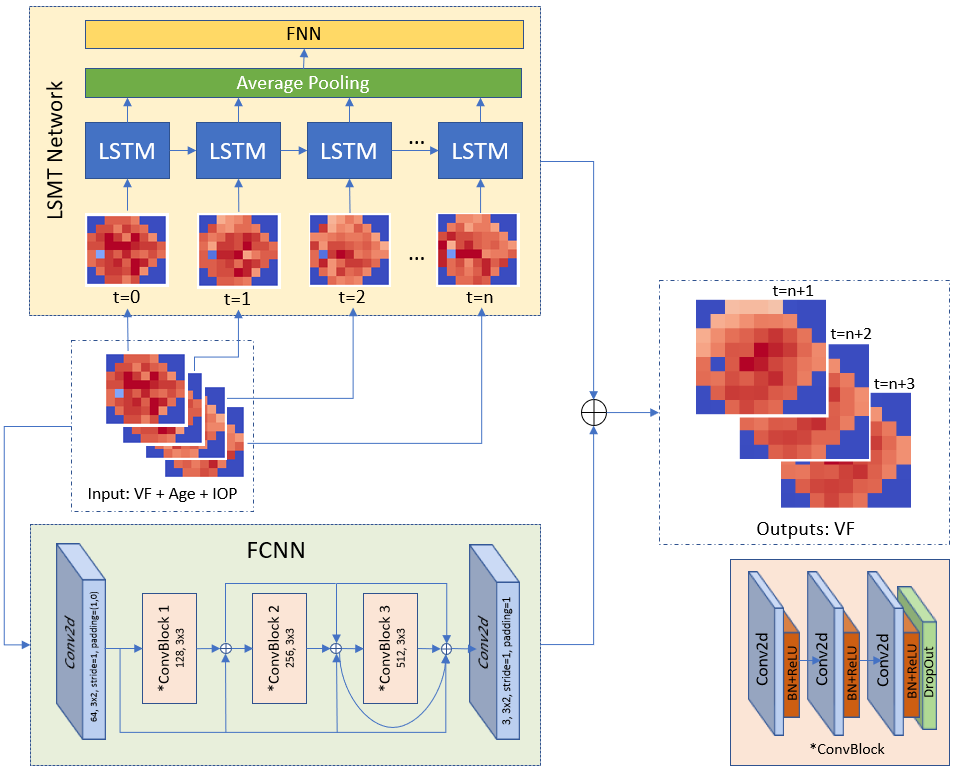
\includegraphics[width=\textwidth]{nn_struct}	\caption{Proposed neural network structure}
		\label{fig:nn_struct}
	\end{figure}

	\item February: Fix current issues present in the algorithm implementation and evaluate network performance against other methods.
	
	\item March: Preliminary testing of designed network on the collected Toronto dataset.
	
\end{itemize}



%% This adds a line for the Bibliography in the Table of Contents.
\addcontentsline{toc}{chapter}{Bibliography}
%% *** Set the bibliography style. ***
%% (change according to your preference/requirements)
\bibliographystyle{IEEEtran}
%% *** Set the bibliography file. ***
%% ("thesis.bib" by default; change as needed)
\bibliography{thesis}

%% *** NOTE ***
%% If you don't use bibliography files, comment out the previous line
%% and use \begin{thebibliography}...\end{thebibliography}.  (In that
%% case, you should probably put the bibliography in a separate file and
%% `\include' or `\input' it here).

\begin{appendices}
	\chapter{Algorithms} \label{chapter:code}

\begin{center}

\captionof{algorithm}{CNN LSTM Forward Propogation} \label{algo:CNNLSTM}
\begin{algorithmic}[1]
	\Procedure{CNNLSTMForward}{input}
	\State $out \gets 0$ \Comment{Initialize LSTM}
	\State $cell \gets 0$
	\State $list \gets [out]$
	\For{$input_i$ in all inputs} \Comment{LSTM network calculation}
		\State $(out, cell) \gets \textrm{LSTM}(input_i, out, cell)$
		\State Append $out$ to $list$
	\EndFor
	\State $\overline{out} \gets \textrm{mean}(list)$ \Comment{LSTM average pooling}
	\State $out_{LSTM} \gets \textrm{linear}(list)$ \Comment{LSTM fully connected layer}
	
	\\
	
	\State $x_{down} \gets \textrm{Conv2d}(input, \textrm{kernel}=(3,2), \textrm{padding}=(1,0))$ \Comment{Down-convolution}
	\State $x_0 \gets \textrm{ReLU}(\textrm{BatchNormalization}(x_{down}))$
	\State $x_1 \gets \textrm{ConvBlock}(x_0) + x_0$ \Comment{Residual Structure}
	\State $x_2 \gets \textrm{ConvBlock}(x_1) + x_0 + x_1$
	\State $x_3 \gets \textrm{ConvBlock}(x_2) + x_0 + x_1 + x_2$
	\State $out_{CNN} \gets \textrm{Conv2d}(x_3, \textrm{kernel}=(3,2), \textrm{padding}=(1,1))$ \Comment{Up-convolution}
	
	\\
	
	\State \Return {$out_{LSTM} + out_{CNN}$}
	
%		\BState \emph{top}:
%		\If {$i > \textit{stringlen}$} \Return false
%		\EndIf
%		\State $j \gets \textit{patlen}$
%		\BState \emph{loop}:
%		\If {$\textit{string}(i) = \textit{path}(j)$}
%		\State $j \gets j-1$.
%		\State $i \gets i-1$.
%		\State \textbf{goto} \emph{loop}.
%		\State \textbf{close};
%		\EndIf
%		\State $i \gets i+\max(\textit{delta}_1(\textit{string}(i)),\textit{delta}_2(j))$.
%		\State \textbf{goto} \emph{top}.
	\EndProcedure
	
	\\
	
	
	\Procedure{ConvBlock}{x}
	
	\State $x \gets \textrm{Conv2d}(x, \textrm{kernel}=(3,3), \textrm{padding}=(1,1))$ 
	\State $x \gets \textrm{BatchNormalization}(\textrm{ReLU}(x))$
	\State $x \gets \textrm{Conv2d}(x, \textrm{kernel}=(3,3), \textrm{padding}=(1,1))$
	\State $x \gets \textrm{BatchNormalization}(\textrm{ReLU}(x))$
	\State $x \gets \textrm{Conv2d}(x, \textrm{kernel}=(3,3), \textrm{padding}=(1,1))$
	\State $x \gets \textrm{BatchNormalization}(\textrm{ReLU}(x))$
	
	\State $x \gets \textrm{Dropout}(x)$
	
	\State \Return {$x$}
	
	\EndProcedure
\end{algorithmic}
\end{center}





\end{appendices}

\end{document}
